План на лекцию:
\begin{enumerate}
    \item Система линейных уравнений в регулярных выражениях.
    \item Быстрый алгоритм минимизации.
    \item Анализ свойств языков.
\end{enumerate}

\subsection{Система линейных уравнений в регулярных выражениях.}

Пусть $\alpha$ и $\beta$ - регулярные выражения

$L = \alpha L + \beta $

\thmm{Лемма:} $\alpha^*\beta$ - решение. Очевидно

\thmm{Теорема.}

$\varepsilon \not \in \alpha \Rightarrow \alpha^*\beta $ --- единственное решение.

$\varepsilon \in \alpha \Rightarrow L = \alpha^*\beta \cup N$ - решение, для $\forall N \subset \Sigma^*$.

\textbf{Доказательство:}
\begin{enumerate}
    \item $\varepsilon \not \in \alpha$:

    База индукции: $|x|= 0, x \in L \Rightarrow x\in \alpha L+\beta \Rightarrow x\in \beta \Rightarrow x\in \alpha^* \beta$.

    ИП. Пусть для всех $|y|<|x| \Rightarrow y \in a^*\beta$.   $x\in L \Rightarrow x\in\alpha L + \beta:$ 
    \begin{enumerate}
        \item $x\in \beta \Rightarrow x\in \alpha^* \beta$
        \item $x \in \alpha L \Rightarrow 
        x = yz,y\in \alpha, z \in L$, $|z|<|x|$, откуда по индукции $x\in \alpha^* \beta$
    \end{enumerate}
    \item $\varepsilon \in \alpha$, $\beta \subset L \Rightarrow \alpha \beta \subset L \Rightarrow \ldots \Rightarrow \alpha^* \beta \subset L$.

    $\forall N: N \subset \alpha N$
\end{enumerate}

\hfill Q.E.D.

Теперь решим систему уравнений. Пусть $X_1,X_2,\ldots, X_n$ - неизвестные языки:
$$\begin{cases}
    X_1 = \alpha_{11}X_1 + \alpha_{12}X_2 + \ldots + \alpha_{1n}X_n  + \beta_1\\
    X_2 = \alpha_{21}X_1 + \alpha_{22}X_2 + \ldots + \alpha_{2n}X_n + \beta_2
\\
\vdots \\
X_n = \alpha_{n1}X_1 + \alpha_{n2}X_2 + \ldots +\alpha_{nn}X_n + \beta_n
\end{cases}$$
Мы тут не можем перенести в левую часть, потому что у нас нет вычитания языков. $\varepsilon \not \in \alpha_{ij}$.

Берем первое уравнение. Возьмем теорему, у нас единственное решение

$X_1 = \alpha_{11}^* (\alpha_{12}X_2 + \alpha_{13}X_3 + \ldots + \alpha_{1n}X_n  +\beta)$

Подставим во второе. Повторим аналогично, как с $A_1$ с $X_1$ и так далее.

Благодаря прошлому мы можем вот таким образом искать регулярное по автомату.

\begin{center}
    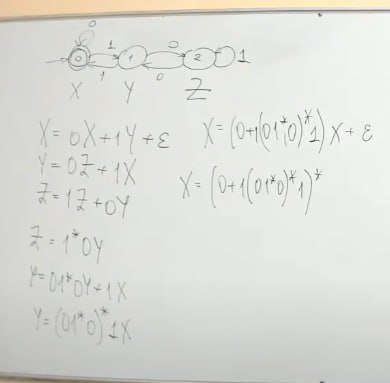
\includegraphics[width = 8cm]{assets/10_2_1.jpg}
\end{center}

\subsection{Алгоритм анализа регулярных языков.}

\thmm{Теорема:} 

Пусть $A,B$ - регулярные языки. $\varphi: \Sigma^* \rightarrow P^*$ - линейная.

$A \cup B,\varphi(A), \varphi^{-1}(A) = \{x|\varphi(x)\in A\}$ - регулярные языки.

\textbf{Доказательство:}

\uline{Докажем $A \cup B$:}

Введем \deff{произведение автоматов} $A \times B$: 

$Q_A \times Q_B: \delta(\langle u_A,u_B\rangle) = \langle \delta_A(u_A,c), \delta_B(u_B,c) \rangle$. $s = \langle s_A, s_B\rangle$, $T = \{\langle t_A,t_B\rangle| t_A \in T_A. t_b \in T_b\}$. 

Заметим, что такое произведение задает объединение автоматов.

\uline{Докажем $\varphi(A)$:}

Возьмем автомат соответствующий $A$, заменим все ребра на $\varphi(c)$(тк по условию нам могут выдавать слова, то возможно на ребре будет записано слово, если так, то построим посимвольную цепочку). Откуда есть автомат $\Rightarrow$ регулярный.

\uline{Докажем $\varphi^{-1}(A)$}

Возьму автомат для $A$. Посмотрю пути из $u,v$, которые по $\varphi(c)$ и на новом автомате между $u,v$ проведу ребро с $c$. Откуда есть соотв. автомат $\Rightarrow$ регулярный.

\subsection{Алгоритм минимизации.}

\thmm{Алгоритм Хопкрофта.}

Алгоритм основан на итеративном разбиении множества состояний на группы эквивалентности.

Начальное разбиение: Все состояния разбиваются на две группы: принимающие состояния (те, которые являются конечными) и непринимающие состояния.

На каждой итерации алгоритм пытается разбить существующие группы эквивалентности на более мелкие, если обнаруживает, что состояния внутри группы ведут себя по-разному для некоторого входного символа.

Назовем $A,B$ - согласованны, если из $B$ все ребра ведут либо в $A$, либо не в $A$.

Цель: Добиться, что все пары согласованны.  
